\chapter{Discussão de resultados}


\section{Teste com somente uma atividade}
\par Para verificar a capacidade de otimização do algoritmo, foi realizado um teste com apenas uma atividade,
de forma que se pudesse prever a melhor solução, para poder verificar a eficiência do algoritmo. Para tal foi 
cadastrado então um processo, criando-se apenas uma atividade para este, conforme mostra a Figura abaixo:

\begin{figure}[h!]
	\centerline{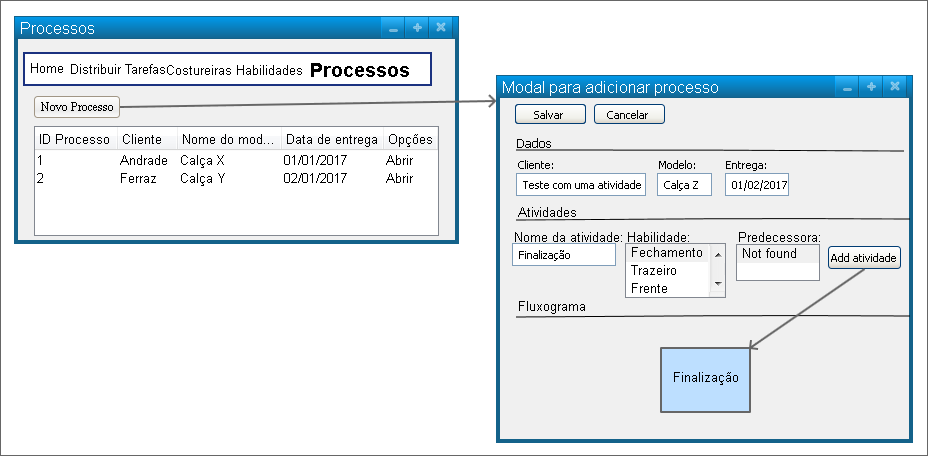
\includegraphics[scale=0.4]{./imagens/test_case_1.png}}
	\caption[Caso de teste]
	{Caso de teste com uma atividade \textbf{Fonte:} Desenvolvido pelos autores}
	\label{fig:exemplo1}
\end{figure}

\par Para a atividade de finalização, atribuída ao processo na Figura acima, foram cadastradas 5 costureiras e seus respectivos
tempos para fazer tal atividade, conforme mostra a Figura abaixo:

\begin{figure}[h!]
	\centerline{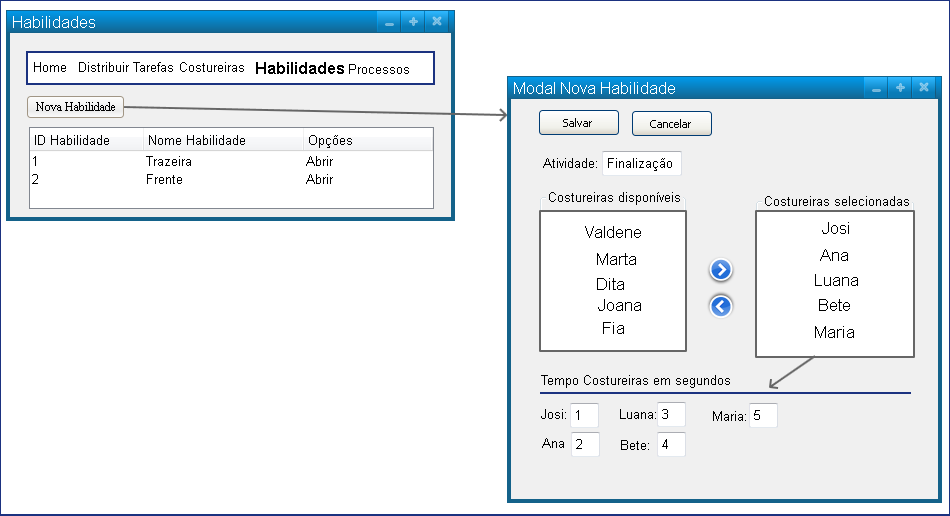
\includegraphics[scale=0.4]{./imagens/test_case_1_habilidades.png}}
	\caption[Caso de teste Habilidade]
	{Cadastro da habilidade e associação das costureiras \textbf{Fonte:} Desenvolvido pelos autores}
	\label{fig:exemplo1}
\end{figure}

\par Feito isso foi iniciado então o processo de distribuição das atividades, através do menu Distribuição de Tarefas.

